\section{Approach Viability}

In order to verify the applicability of our detector and signature language, we tested the system by looking at several recent CVEs related to XSS. Our objective is two-fold: to verify that our signature language provides the necessary functionality to express an exploit and its patch, and to test our detector against existing exploits.

\subsection{Test methodology}

Our work focuses on WordPress as a study platform: we look at recent CVEs related to WordPress plugins. While this may seem restrictive, there are several reasons why this is a worthwhile endeavour:
\begin{itemize}
	\item WordPress powers 25\% of all websites according to a recent survey  \cite{w3techs}. The same study states that 30.3\% of the Alexa top 1000 sites use WordPress. Thus, we can be confident that our study results will hold true for the average user.
	\item WordPress plugins are very popular among developers (there are currently more than 55,000 plugins \cite{wpplugins}). Due to its user popularity, WordPress is also heavily analysed by security experts. There are currently 286 CVEs related to WordPress in the CVE Details database \cite{cvedetails}. Plugins, specifically, are an important part of this issue, 52\% of the vulnerabilities reported by WPScan are caused by WordPress plugins \cite{wpscan}.
	\item Due to the open source nature of WordPress plugins, we can easily analyze both the client-side HTML, as well as the server-side code that generated it, and use this to reach conclusions about the design of our solution.
	\item Using one framework, we can install many different plugins for the version we want, reproduce attacks, and investigate the conditions under which they happen, without having to install additional software.
\end{itemize}

Even though our study has not focused on other sites, our approach is not limited to a specific framework, and we believe it should generalize to arbitrary webpages, under the assumption that we have a pre-existing notion of a webpage's contents.

In order to achieve a comprehensive test suite, we looked at the 100 most recent WordPress XSS CVEs, as of October 2018. We have chosen to use a CVE database, CVE Details \cite{cvedetails}, as opposed to other databases that include vulnerabilities or exploits, mainly because of reliability. We have been able to find hundreds of verified attacks on WordPress and its plugins using a CVE database, which also usually contain information on how to reproduce them. This provides the perfect platform to analyze XSS attacks and decide whether they can be countered by our approach. 

For each CVE, we set up a Docker container with a clean installation of WordPress 5.2 and installed the vulnerable plugin's version. A few of the CVEs depended on the WordPress version as well, and so we used the required WordPress version for those. We then tried to reproduce the exploit as described by the CVE author. Finally, we analyzed the vulnerable page and wrote a signature to patch the exploit.

\subsection{Results}

\begin{table}[h!]
	\begin{center}
		\begin{tabular}{|c c|} 
			\hline
			Plugin & Installations\\ [1ex] 
			\hline
			WooCommerce  & 5+ million  \\  
			Duplicator & 1+ million \\  
			Loginizer & 900,000+ \\  
			WP Statistics & 500,000+ \\  
			Caldera Forms & 200,000+ \\   
			\hline
		\end{tabular}
		\caption{Most popular studied WordPress plugins}
		\label{table:1}
	\end{center}
\end{table}

Of the initial 100 CVEs, we were able to analyze 76 across 40 affected pages. We dropped 24 CVEs due to reproducibility issues: some of the descriptions did not include a proof of concept of the exploit, and as such, was difficult for us to reproduce; or, the plugin code was no longer available. In some cases, it had been removed from the WordPress repository due to "security issues", which exacerbates the importance of being able to defend against these attacks. This is not to say, however, that our detector would not work for such a CVE, as the author would have a better idea of how the exploit manifests itself, and would therefore be in a better position to write a signature. The plugins we studied averaged 489,927 installations, \ref{table:1} shows the number of installations for the 5 most popular studied plugins. For the vulnerabilities, 27 (35.5\%) could be exploited by an unauthenticated user; 56 (73.7\%) targeted a high-privilege user as the victim, 7 (9.2\%) had a low-privilege user as the victim, the rest affected users of all types.

Many of the studied CVEs included attacks for which there are known and widely deployed defenses. For example, many were cases of Reflected XSS, where the URL reveals the existence of an attack e.g:


$http://[path to WordPress]/wp-admin/admin.php?page=wps\_pages\_page\&page-uri=<script>alert("XSS")</script>$

While Chrome's built-in XSS auditor blocked this request, Firefox did not, and so we still wrote signatures for such attacks. We wrote 59 WordPress signatures in total, which got rid of the PoC exploit when sanitized with one of our three methods. We were able to include several CVEs in some of them because they occurred in the same page and affected the same plugin. Overall, these signatures represent 71 (93.4\%) signed CVEs. The 5 we were not able to sign were due to lack of identifiers in the HTML, which would result in potentially large chunks of the document being replaced. For cases like these, the signature developer can weigh the trade-offs and decide whether the added cost is worth it.

The majority of the 71 signatures maintained the same layout and core functionality of the webpage. However, 12 signatures caused some elements to be rearranged, modifying the page's visual aspect. One caused a small part of the page unusable, due to the sanitization method used (e.g. a table showing user information is now rendered as blank). As with the case of unsigned CVEs, most of the responsibility of maintaining functionality is left to the signature developer, being as precise as possible is key: A full sanitization of the whole HTML string will most likely get rid of any exploits, but will also make the page completely unusable in most scenarios.

While our goal with the signature language is to retain as much information of the webpage as possible after sanitization, we believe that even if a part of the page is now useless, this does not impact the user's experience as much, since most of these exploits manifest themselves in small sections of the HTML. A thorough study with regards to usability is out of scope for this work, but we provide a study on false positives and false negatives in later sections, which is related to this issue.



\iffalse
Because of the binding between CVEs and firewall signatures, ideally, our approach should hold at application level, for example, a webpage running WordPress v. 4.9.8, with plugin WooCommerce v. 3.4.6. Due to the nature of websites and their complex interactions between different parts of their back-end, the assumption that we always have full knowledge of the rendering of the client-side HTML might not hold in practice. Even if this assumption held for every individual website, it might not hold true across different websites using similar infrastructure. Both sites might be running WordPress with the same plugins but each of them might have different client-side modifications that would render our searching method less effective. Figure~\ref{fig:admin_view} gives an example of the admin panel of a WordPress site, the part enclosed in the red box is constant across any website using this plugin (Activity Log). In contrast, Figure~\ref{fig:user_view} shows the user side of this webpage, many elements of this view can be modified directly by the admin as they please.  In light of this, we have conducted a study that demonstrates the applicability of our approach.

\begin{figure}[h]
	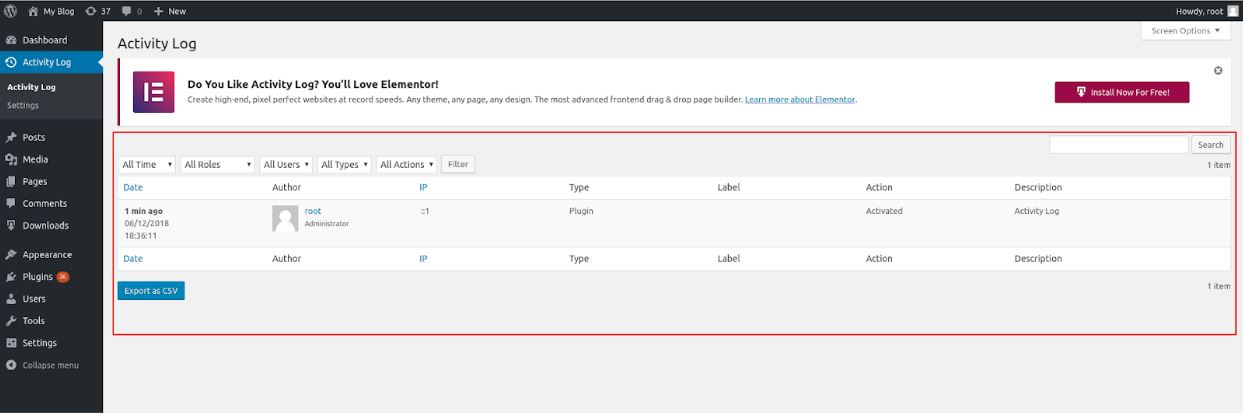
\includegraphics[scale=0.25]{img/admin_view.JPG}
	\caption{Settings page of the Activity Log plugin running on a WordPress website, the section enclosed in red is dictated by the plugin code.}
	\label{fig:admin_view}
\end{figure}

\begin{figure}[h]
	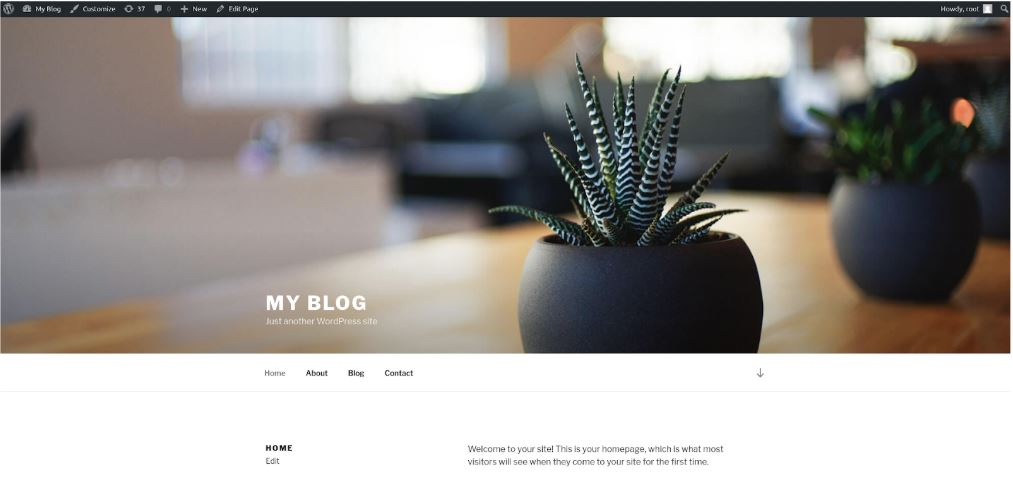
\includegraphics[scale=0.3]{img/user_view.JPG}
	\caption{User view of a WordPress website, much of the layout can be modified by an admin.}
	\label{fig:user_view}
\end{figure}

\subsection{Study Methodology}
In order to achieve a comprehensive study, we have analyzed the 100 most recent CVEs related to XSS attacks, and in particular, to WordPress. We have chosen WordPress because it is widely used, and because it is relatively efficient and easy to reproduce many of the attacks related to it: WordPress plugins are very popular among developers and there's many of these that have been found to be vulnerable to XSS; using one framework, we can install many different plugins for the version we want, reproduce attacks, and investigate the conditions under which they happen, without having to install additional software. We have chosen to use a CVE database, CVE Details \cite{cvedetails}, as opposed to other databases that include vulnerabilities or exploits, mainly because of reliability. We have been able to find hundreds of verified attacks on WordPress and its plugins using a CVE database, which also usually contain information on how to reproduce them. This provides the perfect platform to analyze XSS attacks and decide whether they can be countered by our approach. 

We tagged the analyzed CVEs with four main pieces of information in a yes/no format:
\begin{itemize}
	\item Whether they can be exploited without privileged user authentication: most WordPress sites will allow users to register, and admins of these sites can give increasingly higher privileges to them. Many exploits rely on the fact that the attacker has enough privileges to, for example, submit a post or change some website configurations. As such, we have decided to mark whether an attack requires the user to have high privileges or could just be unauthenticated or have the most basic level of registration. 
	\item Whether the attack manifests itself on an admin-only view (TODO: maybe change this to "an identifiable URL or path, since we are also tagging based on URL and a lot of the CSRF and reflected exploits occur on otherwise 'useless' URLs"): As discussed earlier, our approach relies on very specific knowledge of what the HTML document should look like without any code injections. Many WordPress plugins have an admin-only view for configuration setup where XSS manifests itself. These are of particular interest because these views do not change across different installations of the plugin, that is, different websites using the same plugin will display the same HTML in these views, and so our approach will be easier to apply.
	\item Whether the attack manifests itself on a user-only view (TODO: maybe change this to a non-identifiable view, i.e. placement of elements could vary across different sites, etc.): Like before, many XSS attacks on WordPress may only manifest themselves on the user side of the website, thus, these are likely to vary across different webpages, even if the attack is caused by a WordPress plugin. However, it's worth mentioning that even if this is the case, all might not be lost, as the attack might happen in a very specific HTML context related to the WordPress plugin.
	\item Whether the attack manifests itself through some HTML element (TODO: I feel like this one is useless at this point, but might be worth mentioning the case of non-identifiable pieces of the HTML. Our language is quite expressive, it even lets you specify the position of a certain element, so even for elements that occur several times in the HTML, our approach will still work, but it might be harder and more tedious to do): Sometimes an XSS attack does not have enough context around and is not tightly linked to the HTML document. Attacks that are not related to HTML are not usually covered by our approach. We might be able to use some heuristics for simpler attacks, like URL filtering, but in general we do not expect to be able to guard against these.
\end{itemize}

\subsection{Study Results}

We classified 83 CVEs from our original 100. We dropped 13 of them due to insufficient information in the CVE descriptions to get any meaningful analysis, or because the plugin code was no longer available. In some cases, the plugin had been removed from the WordPress repository due to "security issues", which exacerbates the importance of being able to defend against these attacks.  

The plugins we studied averaged 489,927 installations (min: 10, max: 5 million). Table~\ref{table:1} reports our main results according to our discussed methodology. It is clear from the results that our approach applies to a majority of the studied CVEs. Of particular importance are the first three reported figures.

 A 37\% in "No Authentication" implies that a large number of attacks can be realized by an outsider, and is an alarming reflection of the current state of browser and application defenses against XSS. 
 
 The "User View Only" represents the hardest scenario for us to defend against XSS, as many of the elements in this view won't persist across different websites. A 11\% here means that only a small minority of plugins won't be able to benefit from our strategy. It is worth noting that we have tagged webpages according to this criterion by barely being displayed in the user view, however, there might still be enough identifying information for the injection  to be defended against, and this number might therefore not be fully representative of the limitations of our approach.
 
  While we report a 71\% in "Admin View Only", in our studies we noted that some of the CVE descriptions were somewhat limited and in some cases weren't accurate in describing where the injection points were rendered. As an example, one CVE explained how an unsanitized parameter could trigger XSS in a specific URL of the admin panel, but we found that there were other parts of the admin panel where the same XSS was being triggered. While we believe that this doesn't pose a big issue since it just counts as a failure of the signature description in the firewall, we note that the actual number of websites that can benefit from our approach might be slightly different. 
 
 Finally, even for plugins where we didn't consider it to be able to be defended against in the admin view, we still report the ones where we believe there is some HTML Context that identifies the injection point and can be used to defend against XSS; however, these might be more prone to false positives and therefore only consider them as a "last resort".

Many of the studied CVEs included attacks for which there are known and widely deployed defenses. For example, many were cases of Reflected XSS, where the URL reveals the existence of an attack e.g:


$http://[path to WordPress]/wp-admin/admin.php?page=wps\_pages\_page\&page-uri=<script>alert("XSS")</script>$

While Firefox didn't block this request, Chrome's built-in XSS auditor did block it. We believe such solutions are important and are complementary to our work, and so we still tagged such attacks as identifiable by our approach, as well as having the ability to detecting them in an extension.

After the initial study, we did a second pass over the analysed CVEs. The purpose of this was two-fold: updating any CVEs we hadn't initially considered applicable, now with a more robust iteration of the signature language and detector; and developing signatures for the described exploits. We were able to write 48 (TODO: update this number) signatures that, when sanitized using DOMPurify, got rid of the injection. Some of the exploits we considered as applicable were not able to be signed. For example, two CVEs had been fixed using an external JavaScript file. For this case, the injection can be easily targeted in the source file. This same thought process applies for other most of the other unsigned CVEs. Another example of unsigned CVEs is the case of a high-privilege user attacking a low-privilege one. While this might be XSS by definition, this type of attack can happen regardless of the existence of XSS, and so we do not consider this our main use-case.

The majority of these signatures maintained the same layout and core functionality of the webpage. However, a small number of signatures rendered parts of the page unusable, due to the sanitization method used (e.g. a table showing user information is now rendered as blank). Most of the responsibility of maintaining functionality is left to the signature developer, being as precise as possible is key: A full sanitization of the whole HTML string will most likely get rid of any exploits, but will also make the page completely unusable in most scenarios.

While our goal with the signature language is to retain as much information of the webpage as possible after sanitization, we believe that even if a part of the page is now useless, this does not impact the user's experience as much, since most of these exploits manifest themselves in small sections of the HTML. A thorough study with regards to usability is out of scope for this work, but we provide a study on false positives and false negatives in later sections, which is related to this issue.


\begin{table}
\begin{center}
	\begin{tabular}{|p{2cm}|p{1.5cm}|p{1.5cm}|p{1.5cm}|} 
		\hline
		No Authentication & Admin View Only & User View Only & HTML Context \\ [1ex] 
		\hline
		31 (37\%) & 59 (71\%) & 9 (11\%) & 78 (94\%) \\  [1ex] 
		\hline
	\end{tabular}
\caption{Study results}
\label{table:2}
\end{center}
\end{table}
\fi